
\documentclass[a4paper, 10pt, conference]{IEEEconf}  
    
\usepackage{verbatim}
\usepackage{graphicx}
\usepackage{pdfpages}
\usepackage{cite}



\setlength{\parskip}{1em}


\title{\LARGE \bf
Final Research Proposal, Project Charter\\Beckhoff PLC Smartphone Sensor Control
}

\author{Marc Alexander Sferrazza, Maen Algharaibeh, Abeer Ali Syed, Divraj Singh% <-this % stops a space
\thanks{*This work was not supported by any organization}% <-this % stops a space
\thanks{Faculty of Mechatronics Engineering, Massey University, Albany, Auckland, New Zealand
        {\tt\small Progress of project: alex1v1a.github.io /Beckhoff-PLC-Project-2017/}}%
}


\begin{document}

\begin{figure}
	\centering
	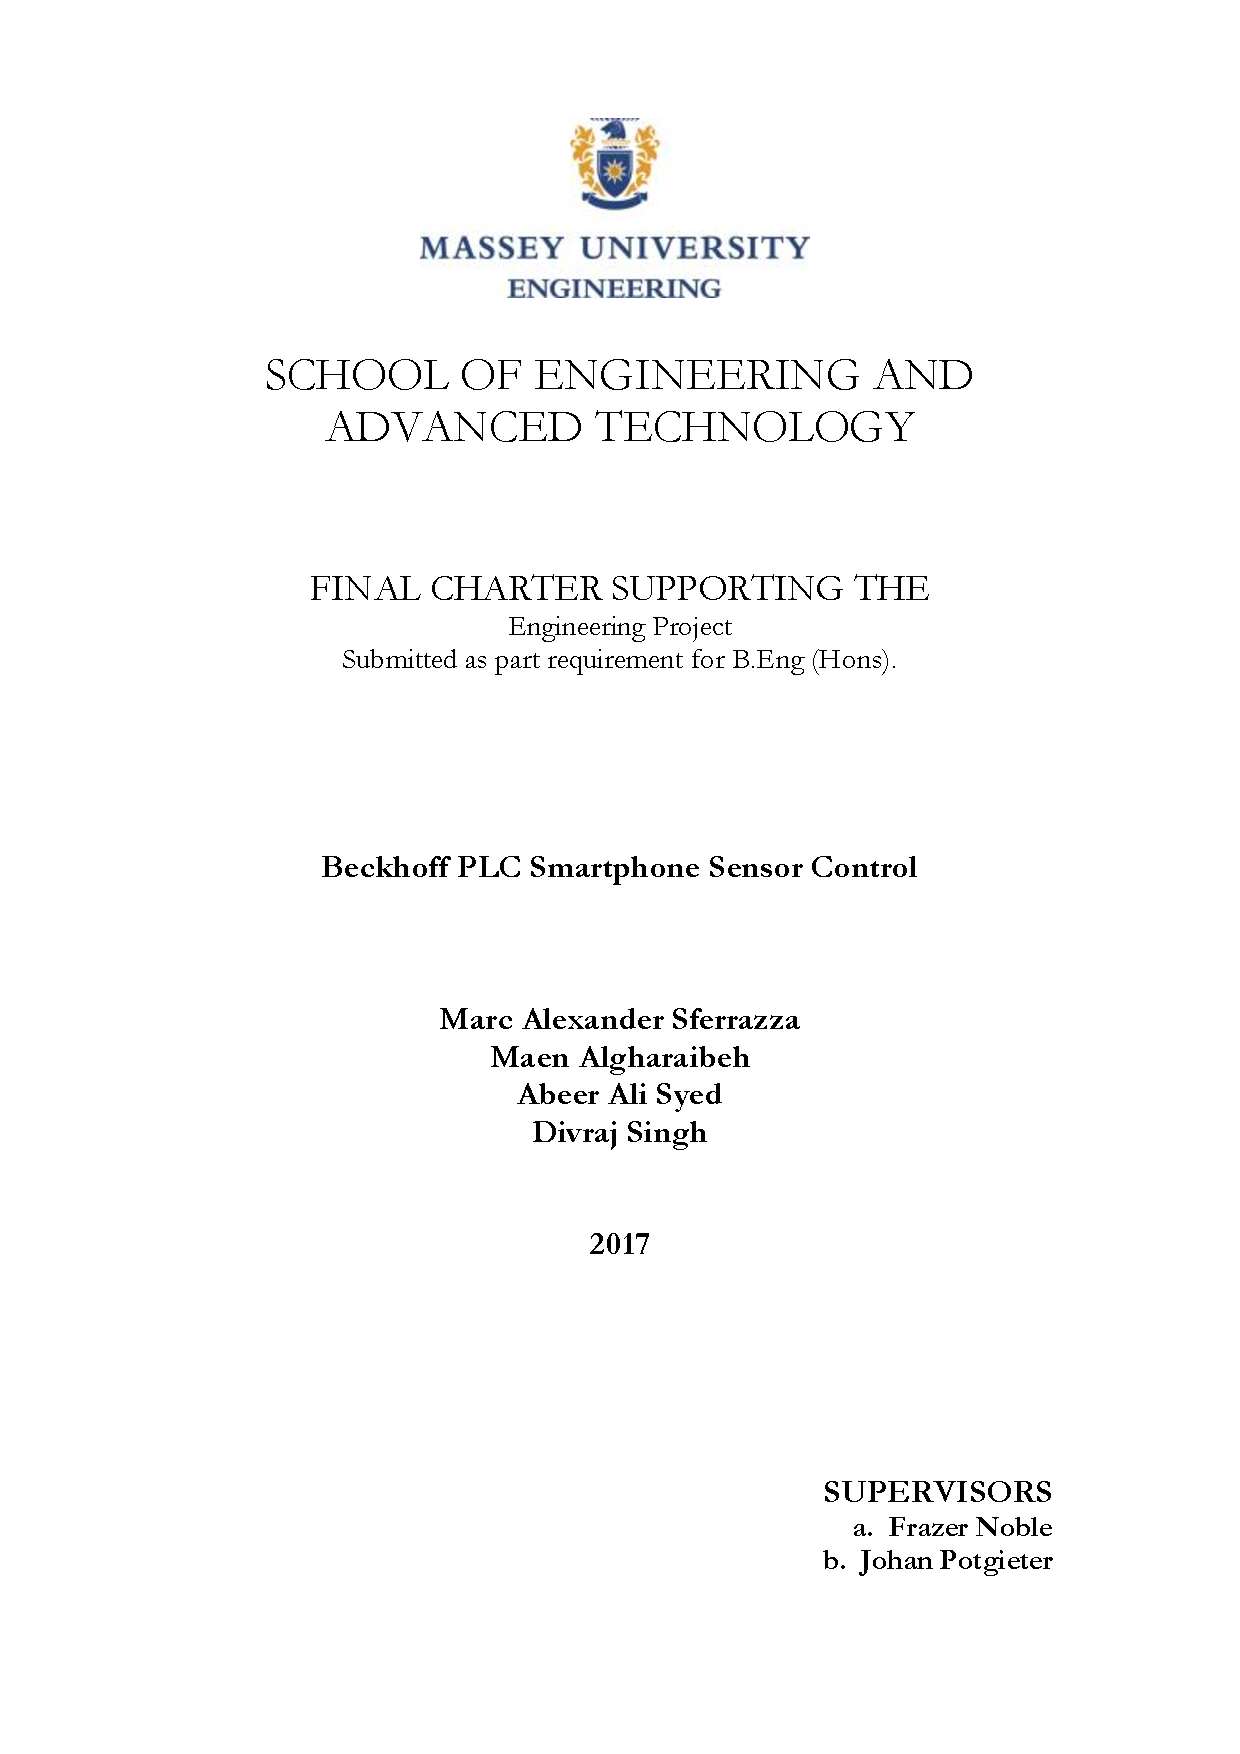
\includepdf[pages=-]{TitlePage.pdf}
\end{figure}

\

\maketitle
\thispagestyle{empty}
\pagestyle{empty}


\begin{abstract}

This report is used to highlight our group's Capstone project for this year. The aim of this project is to create a system which allows the user to read data from a sensor using the Beckhoff Industrial PC remotely via a cloud storage. The PC should also be able to prompt the user with a message if a sensor exceeds a certain limit which then the user can authorise to the system to proceed or cancel the operation.  

This project is going to be carried out under Massey University's Health and Safety guidelines and will be fulfilled with a code of ethics. The project will be supervised by the group's mentors (Dr. Frazer Nobel and Dr. Khalid Arif) and a Beckhoff representative (Omer Naveed).

\end{abstract}


\section{INTRODUCTION}
The purpose of this product is to provide alternative responses, to better improve and achieve daily life tasks with ease, for a more seamless integration of automation. Combining two strong aspects of well developed fields to provide a more efficient system.

With Beckhoff's PLC system based in the TwinCAT environment, and using EtherCAT protocol, communication from a universal compatible sensor module will deliver real-time status on mobile devices; prompting the user with reliable feedback and in some cases giving options to help remotely manage the situation, rather than required manual intervention.

\section{BACKGROUND}
In intelligent factories, machines and products communicate with each other cooperatively driving production. Raw materials and machines are interconnected within an Internet of Things (IoT), the objective is to create a highly flexible individualised and resource friendly mass production which is the vision for the fourth industrial revolution (Industry 4.0).

Taking a look back in history we find that in the 18th century the first steam engines and the use of hydro power began the first revolution in production. In the late 19th century, electric engineering was on the rise, aiding in mass production which indicated the second revolution, the third revolution started in the mid 1970s, electronics and information technology (IT) began to expand rapidly. First set of programmable logic controllers came about in 1969 and production became increasingly based on computer assisted controls. The fourth industrial revolution is still a vision which experts believe will be possible within the next 20 years. All devices, machines and materials within an Intelligent factory will be equipped with sensors and communication technology which will enable them to connect, communicate and control each other cooperatively. 

Beckhoff Automation is an internationally acting company located in Verl Westphalia, Germany with subsidiaries in 34 other countries and over 3000 employees worldwide. Established in the year 1980 as a business unit of the Electrik Beckhoff GmbH, an electrical installation and retail company which was founded in 1953 by Arnold Beckhoff Senior. The company manufactures automation technology in different performance categories ranging from single components up to system solutions. Focusing primarily on PC based control technology with the segments industrial PC, Embedded PC, fieldbus components, drive technology and automation software. The Bus terminals and TwinCat automation software are alternatives to traditional control technology and in 2003 the company initiated a real time ethernet for system control called EtherCAT. 

Beyond the scope of conventional control applications, TwinCAT engineering and control software platforms by Beckhoff Automation also supports big data applications such as horizontal and vertical communication, energy data monitoring, power monitoring, condition monitoring and predictive maintenance. Data is accessible from a local infrastructure or a cloud based environment, the aim of this project is to access this data from a cloud based mobile application and issue commands wirelessly over the internet based on what output the user desires.

\subsection{Research Questions}
To develop and implement sensors of which will notify the user over a cloud based app of any faults in the system; then give options as to which steps the user would like to perform in order to resolve the problem. 

Certain situations will require a more specific approach while the case may be issued to a variety of scenarios; therefore the module will have an approach to universally fit industry sensors and allow for further customisation as per the clients needs.

\subsection{Design and Method}
Using Beckhoffs hardware, and PLC TwinCAT software to send warnings and alerts to the user over cloud based hosting or a site of sorts. After translating the data, receive the users response of how to address the situation of an issued command if available. 

To achieve this in an effective manner designing a sensory module for industry standard to be universal, and using EtherCAT.

Taking the information from the cloud type server or other form of hosting, then having the information to be displayed and response issued back all via an app from either the iOS or Android devices.

As a basis for this module setup, a use of common standard errors has been applied for testing; some of which sensors include but are not limited to are proximity, force-feedback and or, actuation.


\section{SIGNIFICANCE OF RESEARCH}

\subsection{Stakeholders} 
Dr Frazer Noble alongside Dr Khalid Arif will mentor and supervise our group throughout the duration of the project.

Omer Naveed will be our representative and client from Beckhoff. 

Beckhoff Automation the company is a direct stakeholder for this project as the completed task (if implemented) will directly affect the company's sales.

Massey University are the main financial investors for this project, giving our group a budget of \$1000 to cover costs of raw materials and production.

Companies involved within the automation industry such as Seimens and John Brooks alongside companies involved in large production processes such as Coca-Cola and Fonterra would be considered stakeholders as the final result of this project may affect their production line.

Beckhoff PLCs and the TwinCAT software is used alongside multiple sensors, therefore companies involved in supplying these sensors such as Schneider, SenSys and many others would be considered direct stakeholders. 

Towards the end of the project a cloud based mobile application would need to be developed making companies like Apple and Android our stakeholders as the phone application would need to be published to the official online app store.

Startup firms looking to automate their production processes would also be considered stakeholders as they may wish to have their production line maintained from a mobile cloud based application.

Workers which may be made redundant due to this new automation process or workers which would need to be employed to set up and maintain the control system would also be part of the stakeholders.

\subsection{Ethics}

To make sure this project is fulfilled a code of ethics must be place to refer to. Each member of the team must carryout each task with a high level of professionalism. 

How this team makes decisions is a reflection of ethical practice. Consultation with project supervisors and within the team is essential for making decisions for the better development of the project. To achieve this, our team must:

\begin{itemize}
	\item Be thorough and inclusive of all details concerning the decision 
	\item Be objective and not subjective to details central to the project
	\item Be aware of what the decision means or the outcome of the project
\end{itemize}	

Moreover, efficient communication skills are critical to the succession of this project. Team members are expected to:

\begin{itemize}
	\item Clarify information by asking relevant questions.  
	\item Display confidence to better understand given information
	\item Confirm verbal decisions in writing for reference
\end{itemize}	

\subsection{Project Authorization}
This project is authorised by Dr. Frazer Noble(mentor/supervisor), Dr. Khalid Arif(mentor/supervisor) and Omer Naveed (Beckhoff representative). Their responsibilities include, providing the group with constructive feedback, handling financial/funding problems and helping the group with any general enquires. 

\subsection{Limitations}
Knowing the project constraints is an important aspect to the project as it determines the quality of the outcome. It also makes sure that the team stays within the boundaries of the constraints.

\
\
\
\
\
\

For this project the three main constraints are:

\begin{itemize}
	\item Cost
	\item Time
	\item Scope
\end{itemize}	

We are provided with a funding determined by Massey University and Beckhoff and we try not to exceed this constraint. This constraint is challengeable as it can be increased; however, we should try to stay within the initial amount.

Time is a sacrosanct constraint as this project must be completed by the 27th October 2017.

The scope of this project determines how much and how in-depth the project is completed. This is a challengeable constraint as this project is milestone driven (Beckhoff have given us with tasks which need to completed) and the team and mentors can further discuss the scope.

The quality of the outcome of this project is determined by managing these three constraints.

\subsection{Timeline}
This is the initial timeline for the project for the year of 2017.

\begin{figure}[h!]
  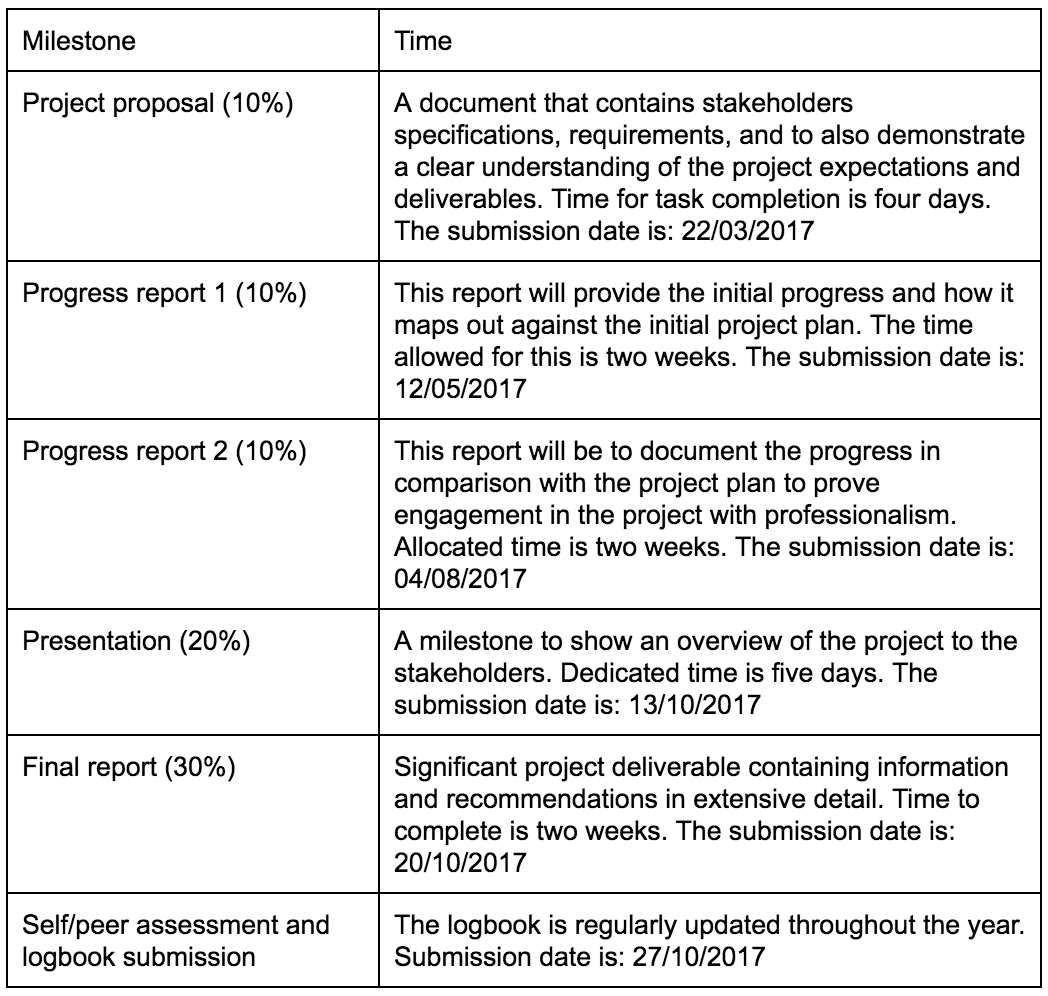
\includegraphics[width=\linewidth]{images/Timeline}
  \caption{Timeline}
  \label{fig:Timeline}
\end{figure}


\section{PROJECT PLAN}

\subsection{Project management}

The project plan is to allocate workload in realisation of strengths of each individual to optimize the team effort and achieve the project deliverables. 

The main and most important resource required for a successful outcome is the performance of each member of the team. The time required for this project is at least 150 hours. This time must be utilized to guarantee the completion of the project.
Another significant resource is the hardware from the Beckhoff company. This includes the PLC computer on which all the programming is carried out.

Also, another major resource is the Beckhoff TwinCAT3 software. This is vital to program the Beckhoff's hardware equipment. The software is downloaded from the Beckhoff website.

In addition, the Massey University workshop. This is a vital resource to provide us with the tools and machinery needed to fabricate any mounting plates and/or housing enclosures needed for this project.

The cost of these resources are as follows (The currency is NZD):
\begin{itemize}
	\item Labour: The time for a team of four experienced graduate students is \$4,000.00
	\item Equipment: Beckhoff hardware \$10,000.00
	\item Workshop Assistance: Assistance and consultation with Paul and/or Sean (Massey University workshop managers) 20 hours is \$1,800.00
\end{itemize}	

{\bf Management Processes}

\begin{itemize}
	\item Reduced overall running costs on the production line decreasing costs of production
More efficient and time managed system
	\item Reduced time spent on troubleshooting and maintaining control systems
	\item Wireless anytime access to the production process allowing maintenance and actions to be carried out without having someone physically drive out on site
	\item Increase in demand of Beckhoff products due to the rise of mobile based application
	\item Less petrol and labour costs due to issues being solved through the mobile application leading to a decrease in carbon emissions and costs of production
\end{itemize}	

Any change proposed to the current plan must go through an authorisation process in which a team meeting will take place. All aspects and consequences must be discussed. A vote will be carried out to resolve the change. Incase of a split decision, Dr. Frazer Noble, Dr. Khalid Arif (mentors/supervisors) and Omer Naveed (Beckhoff representative) will be consulted to reach the desired goals.

The project consent is not applicable to change. Also other content of this project charter which is not subject to change must be agreed upon by all the team members at the launch of this project. 

\subsection{Project Risks}
\
\begin{figure}[h!]
  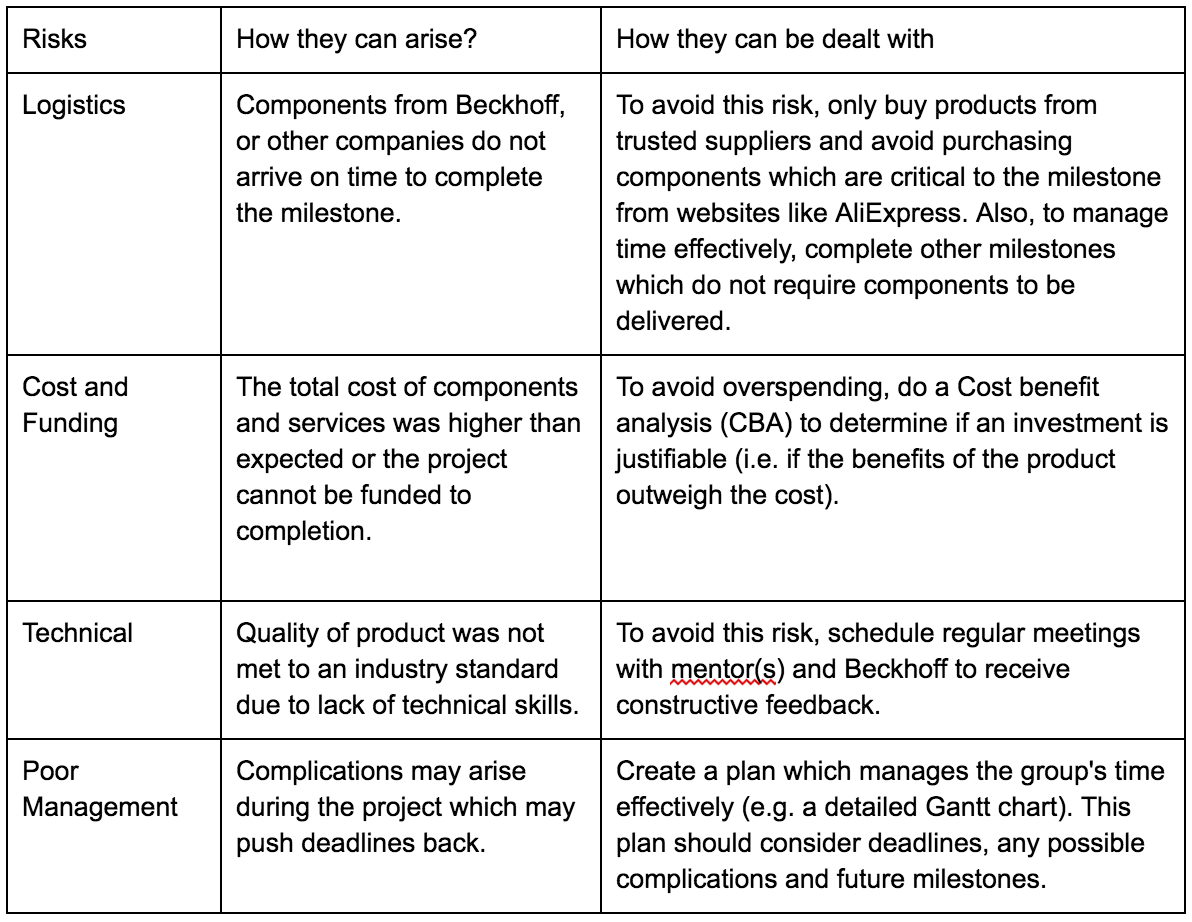
\includegraphics[width=\linewidth]{images/Management}
  \caption{Project Risks}
  \label{fig:ProjectRisks}
\end{figure}

\subsection{Health and safety}
Each member of the team has completed their workshop training and are competent of working with the machinery and tools needed to fabricated enclosures for this project. The team is well aware of using the correct PPE.

However, in chance of any accidents or near misses, members are required to inform workshop staff to receive medical assistance. Team members must also fill out an accident report form. This is so hazards are eliminated or isolated to prevent the repetition of such injuries.

Electrical earthing methods are vital to adopt in this project. This is to prevent electric shocks or any damage to sensitive Beckhoff equipment. 

\subsection{Deliverables}
The main outputs expected from the design are providing real time information to a remote user. A client will be able to select a range of sensors of their choosing to meet the custom requirements. After assembling the sensor module with an actuation unit to control and monitor a system, using EtherCAT the module will send a response to the TwinCAT runtime on the Beckhoff PLC unit in low latency real time. 

After receiving the signal and recording the data on the Beckhoff unit, the information will be sent to the cloud server or other method of hosting (local) of which will push the information to the mobile device (smartphone) displaying an issue or fault and prompting for feedback, else giving the user live analytics of the system and active monitoring.

Using Beckhoffs interface to manage and control the responses in TwinCAT's PLC runtime, for groups of sensors via the EtherCAT protocol; to then be able to relay them via a smartphone app for on-the-go notifications thus further expanding the ease of capability in automation.

If a system reports there is an error or fault e.g. a jamming has occurred in an actuation, the job will present the user on their mobile device with a prompt warning, issuing the command to remedy if possible; this could be subject to the device with error but may have a series of failsafes in place which could fix autonomously rather than manual input.

\subsection{Outcomes}

%{\it Project outcomes}

The project charter is a document that will help foresee the future of the project. Regularly updating this document will help establish the project objectives, deliverables and identify the key stakeholders. This document is crucial for the success of this project as it contributes to keep the team on track and ensure the validity of each milestone. 

\subsection{Results}
{\bf Key project performance criteria (metric)}

\begin{figure}[h!]
  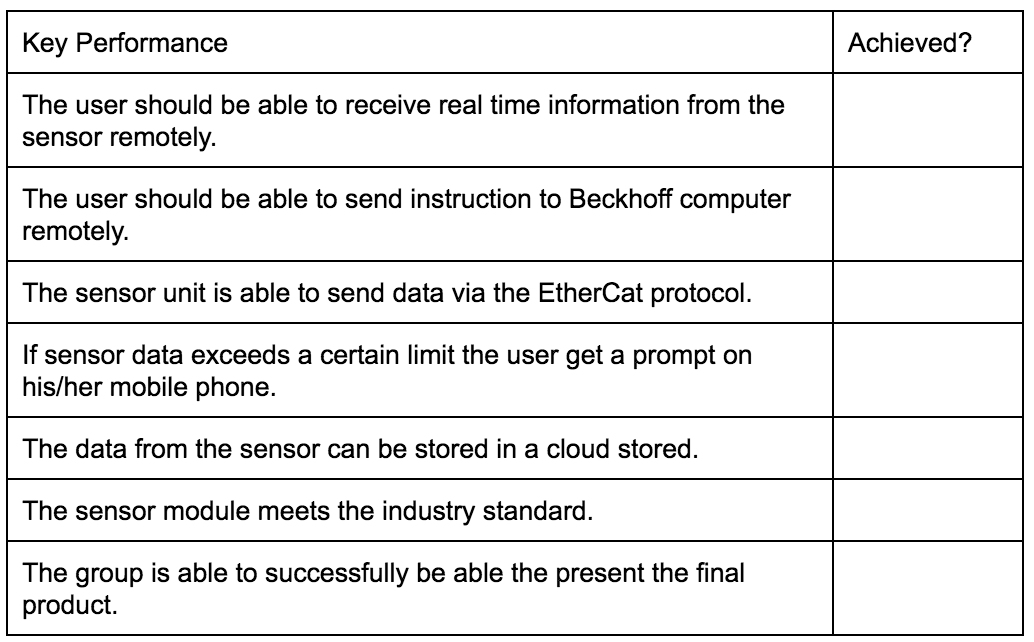
\includegraphics[width=\linewidth]{images/Preformance}
  \caption{Project Risks}
  \label{fig:ProjectRisks}
\end{figure}


\section{CONCLUSIONS}
In conclusion, we aim to provide a solution which will allow the user to efficiently and effectively communicate remotely with Beckhoff PLCs via their mobile device. We will achieve this task with the help of this charter as it will provide us with a clear direction towards milestones and our final goal. This charter will serve as a living document which will be changed and tweaked as the project is further progressed.

\addtolength{\textheight}{-12cm}   % This command serves to balance the column lengths


\section*{APPENDIX}


\section*{ACKNOWLEDGMENT}
The team appreciates Massey University for making this project available for us. The launch of this project could not have been possible without the suggestions and advice of the Massey University staff. Fistly, Associate Professor Johan Potgieter. Also, Dr. Frazer Noble(mentor/supervisor), Dr. Khalid Arif(mentor/supervisor) who have provided us with great insight on this project. 

The team would also like to thank Beckhoff and Omer Naveed (Beckhoff representative) as they have been very helpful in supplying us with the hardware and software needed to start working on the capstone project. 


\nocite{*}
\nocite{key}
\bibliographystyle{ieeetr}
\bibliography{references}

\end{document}
